\documentclass[11pt]{article}

\usepackage[utf8]{inputenc}
\usepackage[spanish]{babel}
\usepackage[pdftex]{graphicx}
\usepackage{url}
%Gummi|065|=)
\title{\textbf{Primer Proyecto Sistemas Operativos}}
\author{Eddy Ramírez \\ Sistemas Operativos \\ I Semestre 2020  }
\date{}
\begin{document}

\maketitle

\section{Motivación}

El propósito de este proyecto es darle familiaridad con el manejo básico de threads y concurrencia. Toda la programación debe realizarse en C sobre Linux, utilizando la biblioteca Pthreads para el manejo de hilos de ejecución. El proyecto debe compilar y ejecutar correctamente en nuestros laboratorios. 

Es importante que se utilice la biblioteca pthread porque está basada en POSIX, el cual es un estándar que todos los sistemas operativos (salvo Windows) utiliza y que por tanto, se vuelve una herramienta útil para poder hacer uso de los servicios del sistema mediante llamadas al sistema o $system$ $calls$.

La idea inicial de tener este proyecto es exponer al estudiante a un espacio donde hayan múltiples procesos y que éstos deban ser calendarizados por el sistema operativo y donde la responsabilidad de administrar su sincronización sea de propia, donde también se deben prevenir los deadlocks.

\section{Objetivos Formativos}

\subsection{Objetivo(s) del curso que respalda el proyecto}
\begin{enumerate}
\item Proporcionar una comprensión sólida de la teoría y práctica básica de los
Sistemas Operativos (objetivo principal).
\item Conocer el funcionamiento de los Sistemas Operativos.
\item Resolver problemas clásicos de los Sistemas Operativos.
\end{enumerate}

%Establecer con claridad la relación entre el proyecto y uno o más de los contenidos del curso. 
\subsection{Contenido(s) del curso que cubre el proyecto}
\begin{itemize}

\item Conceptos Básicos
\subitem Llamadas al sistema
\item Administración de Procesador
\subitem Conceptos
\subitem Comunicación entre procesos
\subitem Threads
\subitem Planificación del CPU
\subitem Sincronización de Procesos
\subitem Bloqueos

\end{itemize}


\section{Especificación del proyecto}
\subsection{El problema del puente estrecho}
Como muestra el siguiente esquema, en cierto sector de la ciudad hay un puente que conecta el sector Este con el sector Oeste.

\begin{figure}[h!]
\centering
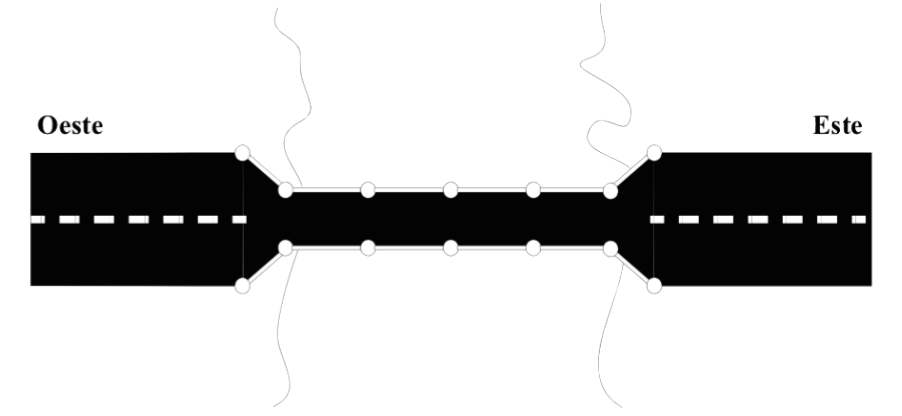
\includegraphics[scale=0.47]{puente.png}
\caption{El Puente}
\label{puenteimg}
\end{figure}

Este puente se considera obsoleto porque sólo tiene el ancho de un autotomóvil, lo cual hace que en un momento dado sólo pueda haber automóviles en uno de los dos sentidos. Hay varias posibilidades para administrar el puente:


\begin{enumerate}
\item Cuando un automóvil llega al inicio del puente, sólo puede utilizarlo si el puente está vacío o si los automóviles que están usándolo viajan en el mismo sentido que él (Oeste-Este o Este-Oeste).

\item Poner semáforos\footnote{En este caso nos referimos a semáforos de tránsito, no a semáforos de Sistema Operativo} coordinados en las dos entradas del puente lo cuales darán paso en cada sentido por una cierta cantidad de segundos.

\item Asignar oficiales de tránsito al puente, los cuales dejarán pasar $K_1$ automóviles ``seguidos'' en un sentido, luego $K_2$ en el otro sentido y así sucesivamente. Si en un momento dado, no hay automóviles moviéndose en el sentido que tiene el puente asignado, pero sí hay automóviles esperando en el otro sentido se les dará el puente a estos últimos aunque no se hayan completado los $K_x$ movimientos en el sentido actual.

\item Se decidió que en todos los casos anteriores si el primer vehículo que
espera por el puente es una ambulancia se le dará prioridad de paso lo antes posible.

\end{enumerate}

Los objetivos de cualquier esquema de administración serán: máxima utilización del puente, mínimo número de automóviles esperando y una asignación justa del puente.


\subsection{Simulación}
Ud. debe escribir una simulación completa del problema descrito. Cada entidad del problema (automóviles, policías, ambulancias, semáforos, etc.) será representado por un thread que actualizarán los puntos apropiados de las estructuras de datos que describan la situación actual.

De alguna manera sencilla el usuario debe indicar cuál de las modalidades de administración del puente desea ejecutar. Se deben desplegar constantemente mensajes en la consola que expliquen que ``está sucediendo'' en el puente.

Deben ser lo más explicativos posibles para entender lo que ocurre.

Los automóviles llegarán al puente siguiendo una distribución exponencial (i.e., los tiempos entre la creación de cada threads que los represente seguirán una distribución exponencial). Además cada uno de ellos tendrá una velocidad ligeramente diferente lo cual afecta el tiempo que requieran para cruzar el puente. Aleatoriamente, cierto porentaje de los autos serán ambulancias.

Dado que la distribución exponencial es integrable, se facilita mucho el calcular los valores exponenciales, a saber:

$$ -media\times log_e(1-r) $$ donde $$0\leq r < 1$$ Nótese que la desigualdad es importante, $r \not = 1$, porque eso indefiniría el logaritmo natural.

\subsubsection{Entrada del programa}

Su programa debe leer los parámetros de ejecución de un archivo de configuración, adonde se definirán detalles tales como la longitud del puente (única para ambos lados), media de la distribución exponencial del tiempo entre llegadas de nuevos automóviles\footnote{independiente para cada sentido}, velocidad promedio de los automóviles\footnote{ídem}, valores para $K_i$\footnote{ídem}, tiempo de duración de la luz verde del semáforo \footnote{ídem} rango inferior y superior de las velocidades de los autos\footnote{ídem}. Todos los parámetros anteriores son independientes para cada sentido del tránsito (salvo la longitud del puente).

Este archivo de configuración debe ser de texto y se sugiere que su programa lea los números, de modo que en el archivo se puedan poner textos con comentarios de qué es cada número, este ejercicio además ayudará a mejorar el manejo del código ASCII (los números van del 30h al 39h o lo que es lo mismo, del 48 al 58 en decimal).


\subsubsection{Restricciones técnicas}
La comunicación y sincronización debe de realizarse por medio de mutex de pthreads y variables en el Data Segment.

Se espera que todos los hilos sean independientes y puedan tomar decisiones \textit{autónomas} dependiendo del modo en que se encuentra.

\subsubsection{Puntos Extras}

Opcionalmente, se puede hacer una representación gráfica (animación) de todo el sistema. Esto implicará puntos extra siempre y cuando TODO lo anterior de la especificación esté completo.

\section{Metodología}
Los estudiantes se deben sentar para diseñar la solución del proyecto y luego se programa. Tal como se indica, deben utilizar la biblioteca pthread, con los mutex y demás recursos necesarios para satisfacer el proyecto.

\section{Rúbrica}
El proyecto va a tener dos rúbricas, la primera sería la nota del programa ($np$) y la segunda sería la nota de la documentación ($nd$). Finalmente la nota del proyecto sería: $\sqrt{np\times nd}$ (es decir, el promedio geométrico deambas notas).\\

NOTA:Si en el programa ocurre algún deadlock, se utiliza $busy-waiting$ o los carros, tránsitos o semáforos no son implementados con hilos, la nota del programa se reduce a la décima parte de lo obtenido por funcionamiento. 

Si alguno de los parámetros del archivo (velocidad, frecuencia de creación, probabilidad de ambulancia, duración de los semáforos, etc) no se recibe \textbf{independientemente} para cada lado de la ciudad, la nota obtenida se reduce a la cuarta parte.

Si faltase algún parámetro de manejar en el puente, la nota se reduce a la mitad. 

Si el puente no se establece con un arreglo de semáforos o no se administran correctamente para que el paso de los carros sea secuencial en el puente, se otorgará sólo un décimo del funcionamiento.\\
\begin{tabular}{|lr|}
\hline
	Producto esperado & Porcentaje\\
	Funcionamiento FIFO & 33\%\\
	Funcionamiento Semáforo & 33\%\\
	Funcionamiento Tránsito & 34\%\\
	\textbf{TOTAL} & 100\%\\
\hline
\end{tabular}
\\\newpage

Para la rúbrica de la documentación, se solicita que sea en Latex, si no se cumple esta premisa, se otorgará un cero.\\
\begin{tabular}{|lr|}
\hline
	Producto esperado & Porcentaje\\
	Portada & 5\%\\
	Introducción y descripción del problema & 5\%\\
	Marco Teórico & 15\%\\
	Descripción de la solución & 15\%\\
	Bitácora de problemas encontrados & 25\%\\
	Conclusiones & 15\%\\
	Descripción de la experiencia (personal) & 15\%\\
	Propuesta de mejoras a la luz de los objetivos & 5\%\\
	\textbf{TOTAL} & 100\%\\
\hline
\end{tabular}



\section{Estimación de tiempo}
\begin{itemize}
\item El proyecto puede ser realizado en grupos de a lo sumo 2 personas
\item Fecha de entrega: 26 de marzo.
\item Estimación de tiempo: Se espera que la parte programada se pueda realizar en 6 horas cada integrante por las dos semanas y que la documentación requiera 2 horas por persona en las dos semanas.
\item Ambos estudiantes deben ser capaces de explicar todos los módulos del proyecto.
\end{itemize}

\section{Aspecto Generales}
\begin{itemize}
\item Formato de entrega: PDF de la documentación y código al correo eddy.ramirez.jimenez@gmail.com y citas de revisión
\item Canal de entrega: Correo edramirez@itcr.ac.cr con el formato correcto del asunto.
\item Penalizaciones: Si no se entrega en la fecha y hora acordada, se reducirán 10 puntos por cada hora.
\end{itemize}


\end{document}
